% Options for packages loaded elsewhere
% Options for packages loaded elsewhere
\PassOptionsToPackage{unicode}{hyperref}
\PassOptionsToPackage{hyphens}{url}
\PassOptionsToPackage{dvipsnames,svgnames,x11names}{xcolor}
%
\documentclass[
  12pt]{article}
\usepackage{xcolor}
\usepackage{amsmath,amssymb}
\setcounter{secnumdepth}{5}
\usepackage{iftex}
\ifPDFTeX
  \usepackage[T1]{fontenc}
  \usepackage[utf8]{inputenc}
  \usepackage{textcomp} % provide euro and other symbols
\else % if luatex or xetex
  \usepackage{unicode-math} % this also loads fontspec
  \defaultfontfeatures{Scale=MatchLowercase}
  \defaultfontfeatures[\rmfamily]{Ligatures=TeX,Scale=1}
\fi
\usepackage{lmodern}
\ifPDFTeX\else
  % xetex/luatex font selection
\fi
% Use upquote if available, for straight quotes in verbatim environments
\IfFileExists{upquote.sty}{\usepackage{upquote}}{}
\IfFileExists{microtype.sty}{% use microtype if available
  \usepackage[]{microtype}
  \UseMicrotypeSet[protrusion]{basicmath} % disable protrusion for tt fonts
}{}
\makeatletter
\@ifundefined{KOMAClassName}{% if non-KOMA class
  \IfFileExists{parskip.sty}{%
    \usepackage{parskip}
  }{% else
    \setlength{\parindent}{0pt}
    \setlength{\parskip}{6pt plus 2pt minus 1pt}}
}{% if KOMA class
  \KOMAoptions{parskip=half}}
\makeatother
% Make \paragraph and \subparagraph free-standing
\makeatletter
\ifx\paragraph\undefined\else
  \let\oldparagraph\paragraph
  \renewcommand{\paragraph}{
    \@ifstar
      \xxxParagraphStar
      \xxxParagraphNoStar
  }
  \newcommand{\xxxParagraphStar}[1]{\oldparagraph*{#1}\mbox{}}
  \newcommand{\xxxParagraphNoStar}[1]{\oldparagraph{#1}\mbox{}}
\fi
\ifx\subparagraph\undefined\else
  \let\oldsubparagraph\subparagraph
  \renewcommand{\subparagraph}{
    \@ifstar
      \xxxSubParagraphStar
      \xxxSubParagraphNoStar
  }
  \newcommand{\xxxSubParagraphStar}[1]{\oldsubparagraph*{#1}\mbox{}}
  \newcommand{\xxxSubParagraphNoStar}[1]{\oldsubparagraph{#1}\mbox{}}
\fi
\makeatother


\usepackage{longtable,booktabs,array}
\usepackage{calc} % for calculating minipage widths
% Correct order of tables after \paragraph or \subparagraph
\usepackage{etoolbox}
\makeatletter
\patchcmd\longtable{\par}{\if@noskipsec\mbox{}\fi\par}{}{}
\makeatother
% Allow footnotes in longtable head/foot
\IfFileExists{footnotehyper.sty}{\usepackage{footnotehyper}}{\usepackage{footnote}}
\makesavenoteenv{longtable}
\usepackage{graphicx}
\makeatletter
\newsavebox\pandoc@box
\newcommand*\pandocbounded[1]{% scales image to fit in text height/width
  \sbox\pandoc@box{#1}%
  \Gscale@div\@tempa{\textheight}{\dimexpr\ht\pandoc@box+\dp\pandoc@box\relax}%
  \Gscale@div\@tempb{\linewidth}{\wd\pandoc@box}%
  \ifdim\@tempb\p@<\@tempa\p@\let\@tempa\@tempb\fi% select the smaller of both
  \ifdim\@tempa\p@<\p@\scalebox{\@tempa}{\usebox\pandoc@box}%
  \else\usebox{\pandoc@box}%
  \fi%
}
% Set default figure placement to htbp
\def\fps@figure{htbp}
\makeatother





\setlength{\emergencystretch}{3em} % prevent overfull lines

\providecommand{\tightlist}{%
  \setlength{\itemsep}{0pt}\setlength{\parskip}{0pt}}



 
\usepackage[]{natbib}
\bibliographystyle{agsm}


\addtolength{\oddsidemargin}{-.5in}%
\addtolength{\evensidemargin}{-1in}%
\addtolength{\textwidth}{1in}%
\addtolength{\textheight}{1.7in}%
\addtolength{\topmargin}{-1in}%
\makeatletter
\@ifpackageloaded{caption}{}{\usepackage{caption}}
\AtBeginDocument{%
\ifdefined\contentsname
  \renewcommand*\contentsname{Table of contents}
\else
  \newcommand\contentsname{Table of contents}
\fi
\ifdefined\listfigurename
  \renewcommand*\listfigurename{List of Figures}
\else
  \newcommand\listfigurename{List of Figures}
\fi
\ifdefined\listtablename
  \renewcommand*\listtablename{List of Tables}
\else
  \newcommand\listtablename{List of Tables}
\fi
\ifdefined\figurename
  \renewcommand*\figurename{Figure}
\else
  \newcommand\figurename{Figure}
\fi
\ifdefined\tablename
  \renewcommand*\tablename{Table}
\else
  \newcommand\tablename{Table}
\fi
}
\@ifpackageloaded{float}{}{\usepackage{float}}
\floatstyle{ruled}
\@ifundefined{c@chapter}{\newfloat{codelisting}{h}{lop}}{\newfloat{codelisting}{h}{lop}[chapter]}
\floatname{codelisting}{Listing}
\newcommand*\listoflistings{\listof{codelisting}{List of Listings}}
\makeatother
\makeatletter
\makeatother
\makeatletter
\@ifpackageloaded{caption}{}{\usepackage{caption}}
\@ifpackageloaded{subcaption}{}{\usepackage{subcaption}}
\makeatother
\usepackage{bookmark}
\IfFileExists{xurl.sty}{\usepackage{xurl}}{} % add URL line breaks if available
\urlstyle{same}
\hypersetup{
  pdftitle={The Noisy Work of Uncertainty Visualisation Research: A Review},
  pdfauthor={Harriet Mason; Dianne Cook; Sarah Goodwin; Emi Tanaka; Susan VanderPlas},
  colorlinks=true,
  linkcolor={blue},
  filecolor={Maroon},
  citecolor={Blue},
  urlcolor={Blue},
  pdfcreator={LaTeX via pandoc}}



\begin{document}


\def\spacingset#1{\renewcommand{\baselinestretch}%
{#1}\small\normalsize} \spacingset{1}


%%%%%%%%%%%%%%%%%%%%%%%%%%%%%%%%%%%%%%%%%%%%%%%%%%%%%%%%%%%%%%%%%%%%%%%%%%%%%%

\date{September 7, 2025}
\title{\bf The Noisy Work of Uncertainty Visualisation Research: A
Review}
\author{
Harriet Mason\\
Department of Econometrics and Business Statistics, Monash University\\
and\\Dianne Cook\\
Department of Econometrics and Business Statistics, Monash University\\
and\\Sarah Goodwin\\
Department of Human Centred Computing, Monash University\\
and\\Emi Tanaka\\
Biological Data Science Institute, The Australian National University\\
and\\Susan VanderPlas\\
Statistics Department, University of Nebraska--Lincoln\\
}
\maketitle

\bigskip
\bigskip
\begin{abstract}
Uncertainty visualisation is quickly becoming a hot topic in information
visualisation. Existing reviews in the field take the definition and
purpose of an uncertainty visualisation to be self evident which results
in a large amout of conflicting information. This conflict largely stems
from a conflation between uncertainty visualisations designed for
decision making and those designed to prevent false conclusions. We coin
the term ``signal suppression'' to describe a visualisation that is
designed for preventing false conclusions, as the approach demands that
the signal (i.e.~the collective take away of the estimates) is
suppressed by the noise (i.e.~the variance on those estimates). We argue
that the current standards in visualisation suggest that uncertainty
visualisations designed for decision making should not be considered
uncertainty visualisations at all. Therefore, future work should focus
on signal suppression. Effective signal suppression requires us to
communicate the signal and the noise as a single ``validity of signal''
variable, and doing so proves to be difficult with current methods. We
illustrate current approaches to uncertainty visualisation by showing
how they would change the visual apprearance of a choropleth map. These
maps allow us to see why some methods succeed at signal suppression,
while others fall short. Evaluating visualisations on how well they
perform signal suppression also proves to be difficult, as it involves
measuring the effect of noise, a variable we typically try to ignore. We
suggest authors use qualitative studies or compare uncertainty
visualisations to the relevant hypothesis tests.
\end{abstract}


\newpage
\spacingset{1.9} % DON'T change the spacing!


\section{Introduction}\label{introduction}

From entertainment choices to news articles to insurance plans, the
modern citizen is so inundated with information in every aspect of their
life it can be overwhelming. In the face of this overflow of
information, tools that effectively reduce piles of information to
simple and clear ideas become more valuable. That is, we need tools that
can sort the signal from the noise.

Among these summary tools, information visualisations are one of the
most powerful as they allow for quick and memorable communication that
allow us to identify quirks in our data that we didn't know to look for.
Datasets such as Anscombe's quartet \citep{anscombe} or the Datasaurus
Dozen \citep{datasaurus, datasaurpkg} show a case where visual
statistics highlight elements of the data that are invisible to the
typical summary statistics. Something as simple as sketching a
distribution before recalling statistics or making predictions can
greatly increase the accuracy of those measures
\citep{Hullman2018, Goldstein2014}.

``Uncertainty visualisation'' is a relatively new field in research.
Early mentions of uncertainty visualisation start to appear in the late
1980s \citep{Ibrekk1987}, with geospatial information visualisation
literature from the early 1990s declaring this to be essential aspect of
any information display \citep{MacEachren1992, Carr1992}.
Figure~\ref{fig-ibrekk} depicts an example of the uncertainty
visualisations discussed in these early papers. Despite kicking off the
field, these papers did not define uncertainty visualisation. This has
led to a lack of consensus on what it means for a graphic to visualise
uncertainty, an issue we will return to later. Therefore, while the
field is considered to be quite new, many of the graphics used for
uncertainty visualisation have been around for much longer. For example,
box plots and histograms display variation which becomes synonymous with
uncertainty when we are using them to depict the variation of an
estimate. Today, there are an abundance of publications on the topic
which makes it timely to construct a review of the field. That is, now
that there is an overwhelming amount of information, it is valuable to
distill it into simple facts. In fact, there have already been several
reviews published but a central piece of discussion is missing.

\begin{figure}

\begin{minipage}{0.33\linewidth}

\centering{

\pandocbounded{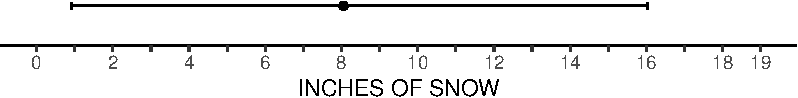
\includegraphics[keepaspectratio]{paper_files/figure-pdf/fig-ibrekk-1.pdf}}

}

\subcaption{\label{fig-ibrekk-1}Picture 1}

\end{minipage}%
%
\begin{minipage}{0.33\linewidth}

\centering{

\pandocbounded{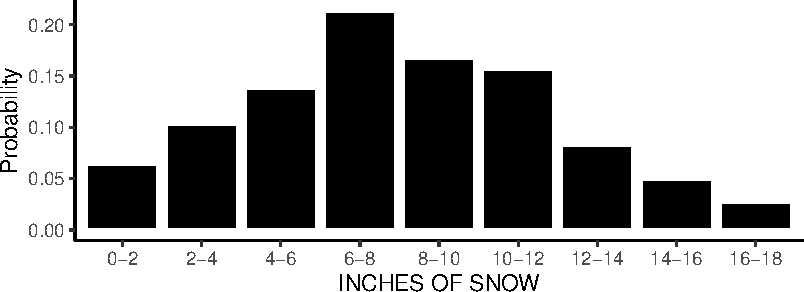
\includegraphics[keepaspectratio]{paper_files/figure-pdf/fig-ibrekk-2.pdf}}

}

\subcaption{\label{fig-ibrekk-2}Picture 2}

\end{minipage}%
%
\begin{minipage}{0.33\linewidth}

\centering{

\pandocbounded{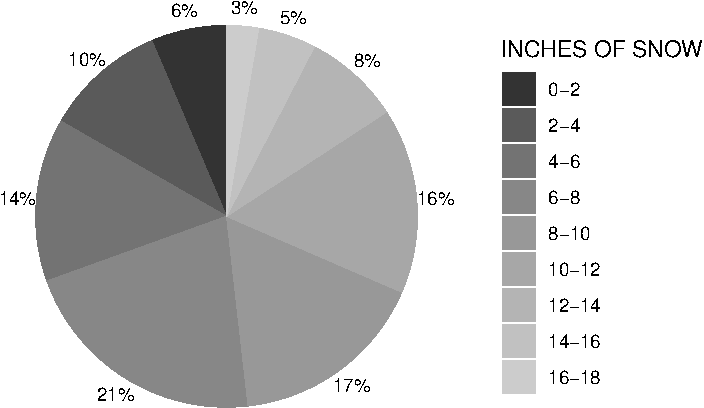
\includegraphics[keepaspectratio]{paper_files/figure-pdf/fig-ibrekk-3.pdf}}

}

\subcaption{\label{fig-ibrekk-3}Picture 3}

\end{minipage}%
\newline
\begin{minipage}{0.33\linewidth}

\centering{

\pandocbounded{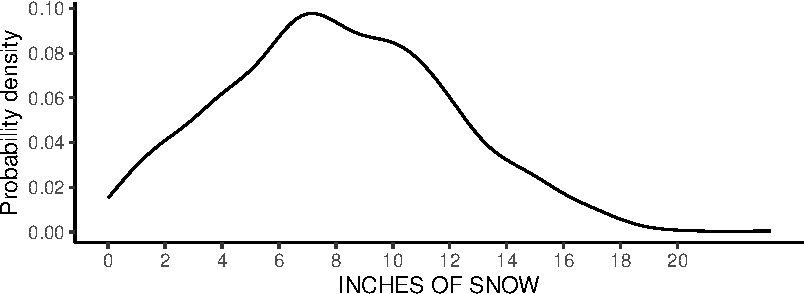
\includegraphics[keepaspectratio]{paper_files/figure-pdf/fig-ibrekk-4.pdf}}

}

\subcaption{\label{fig-ibrekk-4}Picture 4}

\end{minipage}%
%
\begin{minipage}{0.33\linewidth}

\centering{

\pandocbounded{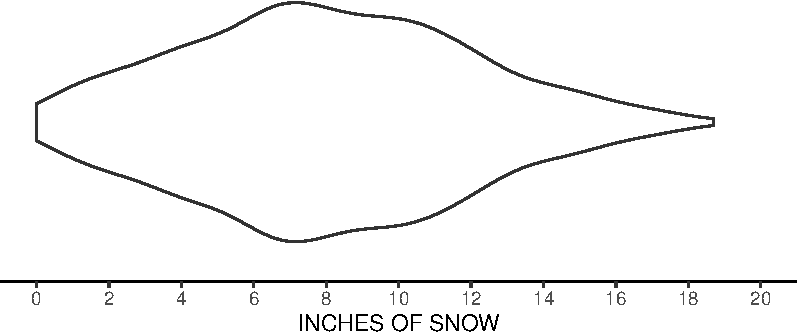
\includegraphics[keepaspectratio]{paper_files/figure-pdf/fig-ibrekk-5.pdf}}

}

\subcaption{\label{fig-ibrekk-5}Picture 5}

\end{minipage}%
%
\begin{minipage}{0.33\linewidth}

\centering{

\pandocbounded{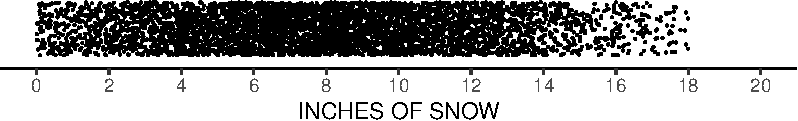
\includegraphics[keepaspectratio]{paper_files/figure-pdf/fig-ibrekk-6.pdf}}

}

\subcaption{\label{fig-ibrekk-6}Picture 6}

\end{minipage}%
\newline
\begin{minipage}{0.33\linewidth}

\centering{

\pandocbounded{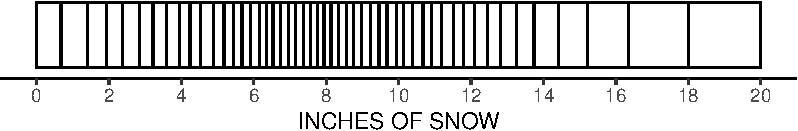
\includegraphics[keepaspectratio]{paper_files/figure-pdf/fig-ibrekk-7.pdf}}

}

\subcaption{\label{fig-ibrekk-7}Picture 7}

\end{minipage}%
%
\begin{minipage}{0.33\linewidth}

\centering{

\pandocbounded{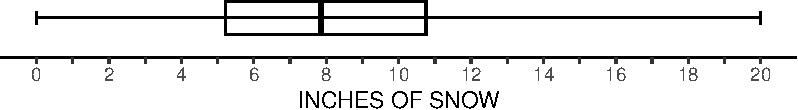
\includegraphics[keepaspectratio]{paper_files/figure-pdf/fig-ibrekk-8.pdf}}

}

\subcaption{\label{fig-ibrekk-8}Picture 8}

\end{minipage}%
%
\begin{minipage}{0.33\linewidth}

\centering{

\pandocbounded{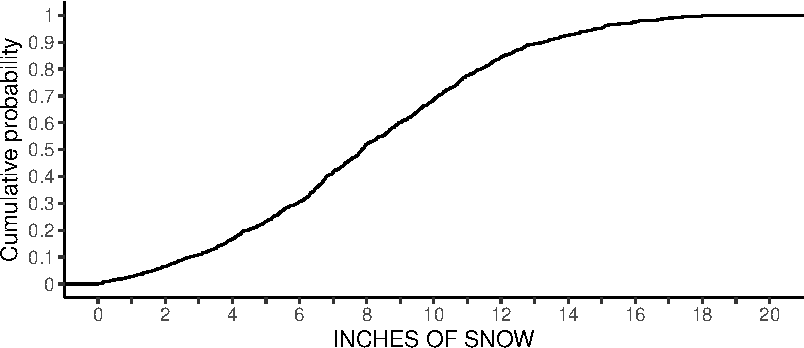
\includegraphics[keepaspectratio]{paper_files/figure-pdf/fig-ibrekk-9.pdf}}

}

\subcaption{\label{fig-ibrekk-9}Picture 9}

\end{minipage}%

\caption{\label{fig-ibrekk}A replication of the uncertainty
visualisations shown by \citet{Ibrekk1987} in one of the earliest
uncertainty visualisation experiments. Several visualisation methods
that are now unpopular (such as the pie chart) are used throughout this
paper.}

\end{figure}%

Reviews on uncertainty visualisation rarely offer tried and tested rules
for effective uncertainty visualisation, but rather, they comment on the
\emph{difficulties} faced when trying to summarise the field.
\citet{Kinkeldey2014} found most experimental methods to be ad hoc, with
no commonly agreed upon methodology, formalisations, or greater goal of
describing general principals. \citet{Hullman2016} noticed there is a
serious noise issue in the data coming from uncertainty visualisation
experiments. She commented on the prevalence of confounding variables
that make it unclear as to what exactly caused a subjects poor
performance on a set of particular questions. Mistakes due to
misunderstanding visualisations, misinterpreting questions, and
incorrectly applying heuristics are all combined into a single error
value. \citet{Spiegelhalter2017} commented that different plots are good
for different things, and disagreed with the goal of identifying a
universal best plot for all people and circumstances.
\citet{Griethe2006} did not identify common themes, but instead listed
the findings and opinions of a collection of papers.
\citet{uncertchap2022} summarised several cognitive effects that
repeatedly arise in uncertainty visualisation experiments, however these
effects were each discussed in isolation as a list of considerations an
author might make rather than an overarching theory of rules for
effective uncertainty visualisation. While these reviews are thorough in
scope, none discuss how the existing literature contribute to the
broader goal of uncertainty visualisation. The problem faced by the
literature is easily summarised with a famous quote by Henri Poincaré.

\begin{quote}
``Science is built up of facts, as a house is built of stones; but an
accumulation of facts is no more a science than a heap of stones is a
house.'' - Henri Poincaré (1905)
\end{quote}

That is to say, despite the wealth of reviews, the field of uncertainty
visualisation remains a heap of stones. There is a mountain of work that
identifies common heuristics found in uncertainty visualisations,
evaluate competing plot designs, or start a theoretical discussion on a
niche aspect of the field. This is important work that needs to be done,
but each of these papers offers up their own bespoke motivation and
methodology, with little reference to the uncertainty visualisation
papers outside their periphery. This becomes even more difficult to
manage when these studies are in conflict. The field is in desperate
need of a unifying theory that can tie this swath of research together.
This review attempts to address this issue by offering a novel
perspective on the uncertainty visualisation problem. That is, we are
going to use the wealth of established stone to construct the
foundations on which we can build a house.

This review is broken into several parts that each reflect a different
approach to uncertainty visualisation. First, we look at graphics that
ignore uncertainty entirely and discuss why uncertainty should be
included at all. Second, we look at methods that consider uncertainty to
be just another variable and discuss the characteristics of uncertainty
that make it a unique visualisation problem. Third, we look at methods
that explicitly combine our estimate and its uncertainty and discuss the
limitations of these approaches. Fourth, we discuss methods that
implicitly include uncertainty by depicting a sample in place of an
estimate. Finally, we discuss how uncertainty visualisations can be
effectively evaluated. When discussing each of these methods, we will
repeatedly return to the \emph{purpose} of uncertainty visualisation and
the effectiveness of each approach in fulfilling that purpose.

\subsection{Spatial example}\label{spatial-example}

There are far too many uncertainty visualisations to exhaustively
discuss them all. Instead we focus on the changes made to a single plot,
the choropleth map. Due to the field's origins and focus in geospatial
information visualisation, there have been a large number of suggested
variations on the choropleth map that allow authors to include
uncertainty. Utilising a single example will help isolate the ideas we
are trying to convey. Therefore, it is important to remember that even
though we focus our discussion on the choropleth map, the theoretical
approach we outline in this review is useful to all uncertainty
visualisations regardless of their application. Additionally, our
examples focus on incorporating uncertainty through colour manipulation,
as that is the key visual channel used in a choropleth map. However, the
methods we discuss go beyond variations in a colour palette. Even though
they are not explicitly shown, visualisations that depict uncertainty
using layers such as position or shape, and more complicated graphics
that incorporate animation or interactivity are also within the scope of
this review. We will use the choropleth maps as a tool to clearly
highlight the costs and benefits of each approach.

Figure~\ref{fig-data} shows the first six rows and the geographical
boundaries of our data set. The temperature variable was generated using
a sine wave, that is
\(Temperature_i = 29-2\cdot{|Latitude_i - \sin{2 \cdot Longitude_i}|}\)
where the \(Longitude\) and \(Latitude\) are the longitude and latitude
of the county's centroid scaled to a standard normal distribution. Each
county's variance is independently, randomly sampled from a uniform
distribution. The low standard errors are drawn from a \(U_{[0,1]}\)
distribution, while the high standard errors are drawn from a
\(U_{[1,2]}\) distribution. As we are dealing with an average, the
sampling distribution would be approximately normal by the central limit
theorem, so each county temperature estimate is assumed to come from a
\(N(Temp_i, SE_{case,i})\). This is the data we will be using in our
spatial uncertainty examples for the rest of the paper.

\begin{figure}

\begin{minipage}{0.50\linewidth}

\centering{

\pandocbounded{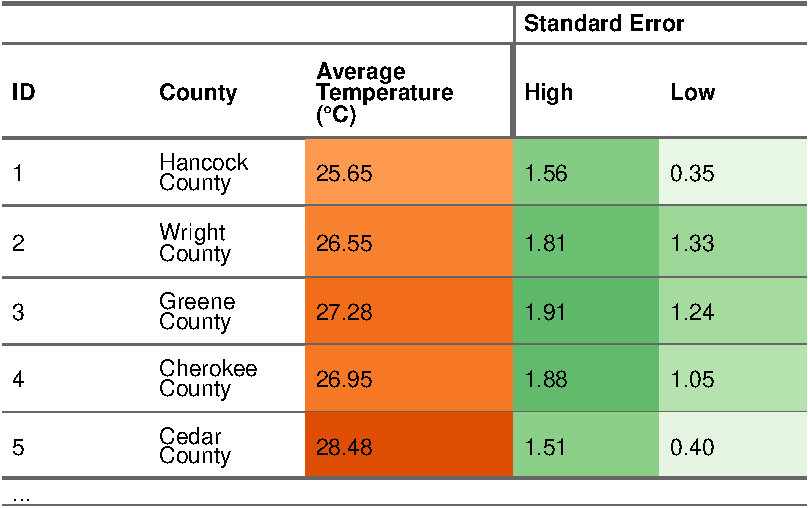
\includegraphics[keepaspectratio]{paper_files/figure-pdf/fig-data-1.pdf}}

}

\subcaption{\label{fig-data-1}Data Table}

\end{minipage}%
%
\begin{minipage}{0.50\linewidth}

\centering{

\pandocbounded{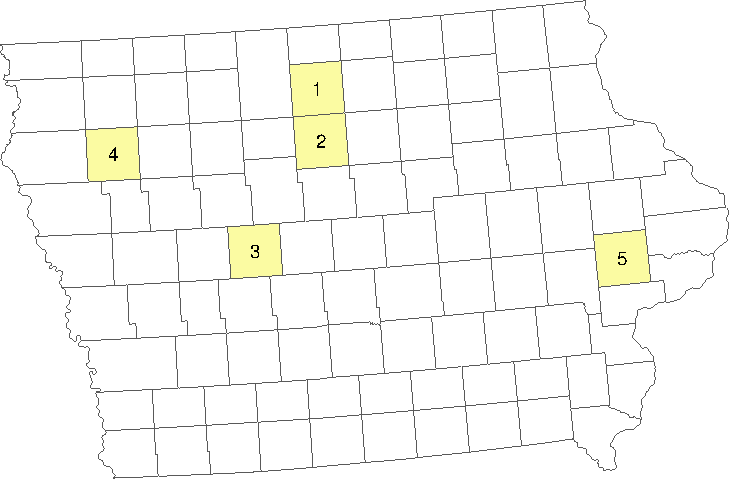
\includegraphics[keepaspectratio]{paper_files/figure-pdf/fig-data-2.pdf}}

}

\subcaption{\label{fig-data-2}Map Boundaries}

\end{minipage}%

\caption{\label{fig-data}The first 5 observations of the data used for
the spatial uncertainty examples along with the boundaries of each
county. The map boundaries are the Iowa county boundaries, however the
`temperature' data is not representative of the average temperature in
Iowa. The temperature and standard error represent the average of the
daily high temperature and the standard error of that average
respectively.}

\end{figure}%

\section{Ignoring uncertainty}\label{ignoring-uncertainty}

A good place to start might be at a deceptively straight forward
question, why should we include uncertainty at all?

\subsection{The choropleth map}\label{the-choropleth-map}

Figure~\ref{fig-choropleth} depicts a choropleth map of the counties of
Iowa. Each of these counties are coloured according to an estimate of
average daily temperature that was generated so that the values followed
a clear spatial trend. The variance of these estimates were simulated
such that the trend accounts for most of the variance in the plot in the
low variance case (so we should expect the trend to be visible) while in
the high variance, there is more variance within each county than
between all the counties, so we should expect it to (at least in some
capacity) overwhelm the spatial trend. Is this aspect of the data and
the spatial data it communicates clear in in the map? Is the strength of
the trend communicated through the visualisation?

\begin{figure}

\begin{minipage}{0.33\linewidth}

\centering{

\pandocbounded{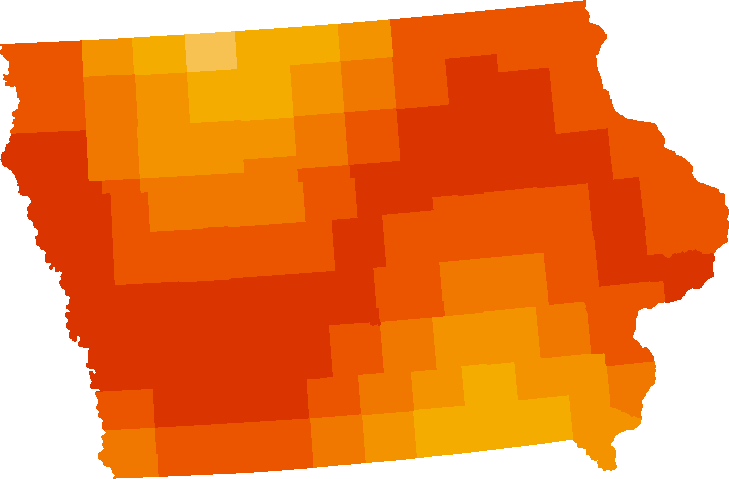
\includegraphics[keepaspectratio]{paper_files/figure-pdf/fig-choropleth-1.pdf}}

}

\subcaption{\label{fig-choropleth-1}Low Variance Data}

\end{minipage}%
%
\begin{minipage}{0.33\linewidth}

\centering{

\pandocbounded{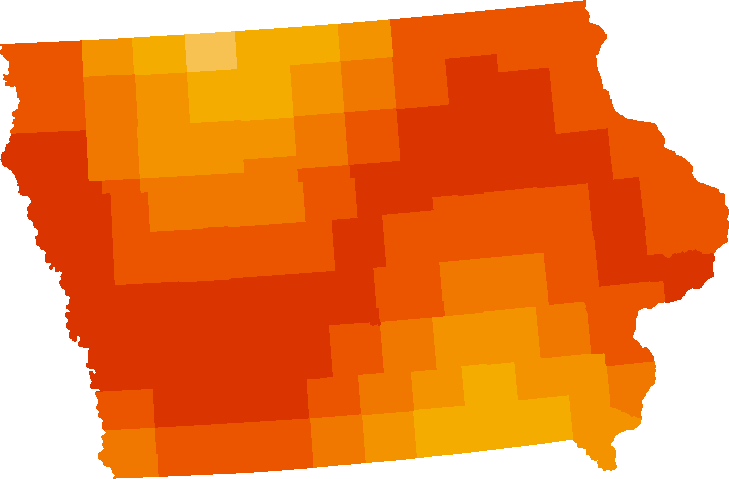
\includegraphics[keepaspectratio]{paper_files/figure-pdf/fig-choropleth-2.pdf}}

}

\subcaption{\label{fig-choropleth-2}High Variance Data}

\end{minipage}%
%
\begin{minipage}{0.33\linewidth}

\centering{

\pandocbounded{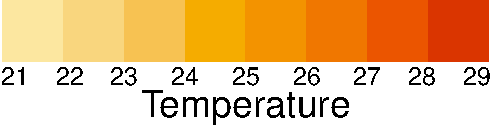
\includegraphics[keepaspectratio]{paper_files/figure-pdf/fig-choropleth-3.pdf}}

}

\subcaption{\label{fig-choropleth-3}Choropleth Palette}

\end{minipage}%

\caption{\label{fig-choropleth}Two choropleth maps that depict the
counties of Iowa where each country coloured acording to a simulated
average temperature. Both maps depict a spatial trend, where counties
closer to the centre of the map are hotter than counties on the edge of
the map. In the low variance condition, the trend accounts for most of
the variation in the data, in the high variance case, the variance on
the temperature estimate accounts for most of the variance. This
distinction is not clear in the map as they both appear identical. The
high variance condition displays a spatial trend that could simply be
spurious, which means the plot is displaying a false conclusion.}

\end{figure}%

\subsection{Signal-suppression}\label{signal-suppression}

Uncertainty visualisation is required for transparency. The two
choropleth maps that appear to be identical in
Figure~\ref{fig-choropleth} highlight the issues with simply electing to
ignore uncertainty. This sentiment appears frequently in the uncertainty
visualisation literature. Some authors suggest uncertainty is important
to include as it communicates the legitimacy (or illegitimacy) of the
conclusion drawn from visual inference
\citep{Correll2014, Kale2018, Griethe2006}. Some authors have said that
uncertainty should be included to degree of confidence or trust in the
data \citep{Boukhelifa2012, Zhao2023}. Some authors directly connect
uncertainty visualisation to hypothesis testing as it ensures the
validity of a statement \citep{Hullman2020a, Griethe2006}, but allows
for a proportional level of trust that is more detailed than the binary
results of a hypothesis test \citep{Correll2014, Correll2018}. Some
authors even go so far as to claim that failing to include uncertainty
is akin to fraud or lying \citep{Hullman2020a, Manski2020}.

This consensus leads us to understand that uncertainty visualisation is
motivated by the need for a sort of ``visual hypothesis test''. A
successful uncertainty visualisation would act as a ``statistical
hedge'' for any inference we make using the graphic. Since the purpose
of a visualisation is to give a quick gist of the information
\citep{Spiegelhalter2017}, this hedging needs to be communicated
visually without the need for complicated calculations. If we refer to
the conclusion we draw from a graphic to be its signal and the variance
that makes this signal harder to identify as the ``noise'', we can
summarise the above information into three key requirements. A good
uncertainty visualisation needs to:

\begin{enumerate}
\def\labelenumi{\arabic{enumi})}
\tightlist
\item
  Reinforce justified signals to encourage confidence in results
\item
  Hide signals that are overwhelmed by noise to prevent unjustified
  conclusions
\item
  Perform tasks 1) and 2) in a way that is proportional to the level of
  confidence in those conclusions.
\end{enumerate}

As Figure~\ref{fig-choropleth} showed, visualisations that are
unconcerned with uncertainty have no issue showing justified signals,
but struggle with the display of unjustified signals. Therefore, we call
this approach to uncertainty visualisation as ``signal-suppression''
since it primarily differentiates itself from from the normal
``noiseless'' visualisation approach through criteria (2). That is, the
main difference between an uncertainty visualisation and a normal
visualisation is that an uncertainty visualisation should prevent us
from drawing unjustified conclusions.

\subsection{Uncertainty as a signal}\label{uncertainty-as-a-signal}

Uncertainty visualisation is not only motivated by signal-suppression,
and we would be remiss if we did not mention these alternative
approaches. Some authors claim the purpose of uncertainty is to improve
decision making
\citep{Ibrekk1987, uncertchap2022, Hullman2016, Cheong2016, Boone2018, Padilla2017}.
Other authors do not describe uncertainty as important for decision
making, but rather explicitly state it as a variable of importance in of
itself \citep{Blenkinsop2000}. While uncertainty can provide useful
information in decision making, it is important to recognise that the
``uncertainty'' in these cases is not acting as uncertainty at all. It
is acting as signal.

This is obvious for the cases where we are explicitly interested in the
variance or error, as we are literally trying to draw conclusions about
an statistic that is used to describe uncertainty. The same is true for
visualisations made for decision making, but it is less overt. This is
easiest to understand with an example.

Imagine you are trying to decide if you want to bring an umbrella with
you to work. An umbrella is annoying to bring with you, so you only want
to pack it if the chance of rain is greater than 10\%. Unfortunately,
your weather prediction app only provides you with the predicted daily
rainfall. Therefore, your decision will be improved with the inclusion
of uncertainty. This is \emph{not} because uncertainty in general is
important for decision making, but because it gives you the tools
required to calculate the \emph{actual} statistic you are basing your
decision on. In this sense, uncertainty is no more special to decision
making than weight is special to a body mass index calculation.

This means the uncertainty visualisations that would perform the best in
decision making would simply display the uncertainty statistic we are
interested in, such as the variance, or probability of an event, using
existing visualisation principles. This is precisely what we observe in
the literature. Figure~\ref{fig-exceed} depicts an exceedance
probability map that was designed as an alternative to the choropleth
map to improve decision making under uncertainty
\citep{Kuhnert2018, Lucchesi2021}. A keen viewer may notice that the
exceedance probability map is actually just a choropleth map, only the
statistic being displayed has changed. We are not sure it is productive
to categorise this visualisation as an uncertainty visualisation.

\begin{figure}

\begin{minipage}{0.33\linewidth}

\centering{

\pandocbounded{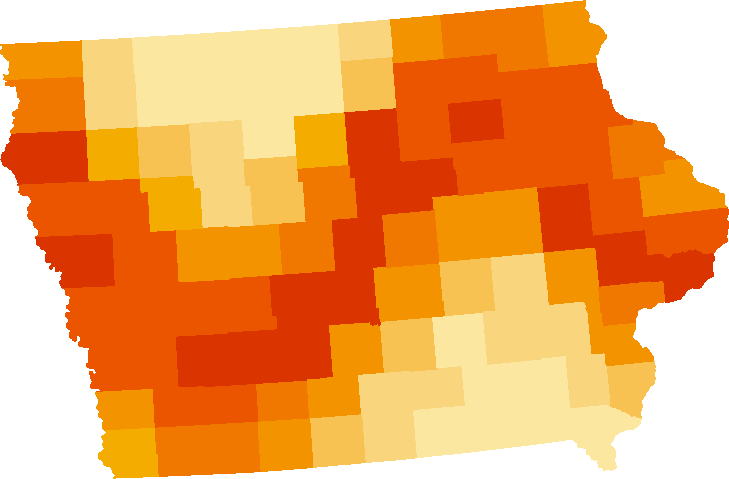
\includegraphics[keepaspectratio]{paper_files/figure-pdf/fig-exceed-1.pdf}}

}

\subcaption{\label{fig-exceed-1}Low Variance Data}

\end{minipage}%
%
\begin{minipage}{0.33\linewidth}

\centering{

\pandocbounded{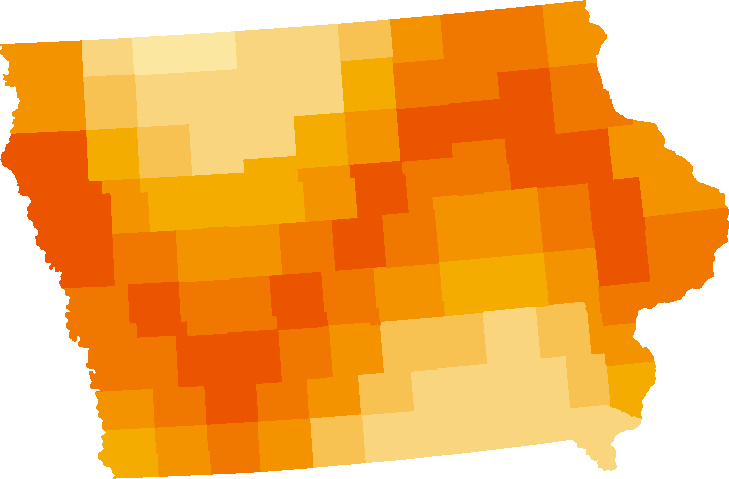
\includegraphics[keepaspectratio]{paper_files/figure-pdf/fig-exceed-2.pdf}}

}

\subcaption{\label{fig-exceed-2}High Variance Data}

\end{minipage}%
%
\begin{minipage}{0.33\linewidth}

\centering{

\pandocbounded{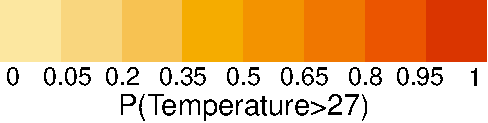
\includegraphics[keepaspectratio]{paper_files/figure-pdf/fig-exceed-3.pdf}}

}

\subcaption{\label{fig-exceed-3}Exceedance Probability Map Palette}

\end{minipage}%

\caption{\label{fig-exceed}An exceedance probability map that depict the
counties of Iowa where each country coloured acording to the probability
that the average temperature exceeds 27. This map is a choropleth map
where the variable of interest is a probability.}

\end{figure}%

There seem to be two different definitions of uncertainty visualisation
floating around in the literature. The first considers \emph{any}
visualisation of error, variance, or probability to be an uncertainty
visualisation. The second believes an uncertainty visualisation is the
output of a function that takes a normal visualisation as an input, and
transforms it to include uncertainty information. The former group
believe the purpose of uncertainty visualisation to provide signal about
a distribution, while the later believe it should act as noise to
obfuscate a signal. The lack of explicit distinction between these two
motivations leaves the literature muddled and reviewers struggle to
understand if uncertainty should be treated as a variable, as metadata,
or as something else entirely \citep{Kinkeldey2014}. This disagreement
creates constant contradictions in what the literature considers to be
an uncertainty visualisation. For example \citet{Leland2005} mentions
that popular graphics, such as pie charts and bar charts omit
uncertainty, and \citet{Wickham2011} suggests their product plot
framework, which includes histograms and bar charts, should be extended
to include uncertainty. However, pie charts, bar charts and histograms
have all been used in a significant number of uncertainty visualisation
experiments \citep{Ibrekk1987, Olston2002, Zhao2023, Hofmann2012}. If
you view an uncertainty visualisation as a function applied to an
existing graphic, then you would not see a pie chart or bar chart as
uncertainty visualisations. These charts are they are yet to have the
uncertainty visualisation function applied to them. If you view an
uncertainty visualisation as any graphic that depicts a statistic then
there are no limitations on which graphics can or cannot be uncertainty
visualisations.

When we use the term uncertainty visualisation to refer to graphics that
simply communicate a variance or probability, we are classifying
visualisations by the data they display, not their visual features.
Graphics, just like statistics, are not defined by their input data. A
scatter plot that compares mean and a scatter plot that compares
variances are both scatter plots. Given that there is no special class
of visualisation for \emph{other} statistics (such the median or
maximum) there is no reason to assume visualisations that simply depict
a variance, error, or probability to be special. Some authors implicitly
suggest that visualisations of variance or probability are
differentiated due to the psychological heuristics involved in
interpreting uncertainty \citep{Hullman2019}. While it is true that
heuristics lead people to avoid uncertainty \citep{Spiegelhalter2017},
there is no evidence that this psychological effect translates to issues
with the visual representation of uncertainty. Again, given that we do
not make these same visual considerations for other variables that
elicit distaste or irrational behaviour, there is no reason to assume
this is what makes uncertainty visualisation so special.

This leads us to the conclusion that the visualisations made for the
purpose of displaying information about uncertainty statistics are not
uncertainty visualisations. These graphics are just normal information
visualisations, and authors can follow existing principles of graphical
design. We focus on the perspective that uncertainty visualisation
serves to obfuscate signal, and an uncertainty visualisation is a
variation on an existing graphic that gives it the ability to suppress
false signals.

Of course, there is nothing wrong with explicitly visualising variance,
error, bias, or any other statistic used to depict uncertainty as a
signal. Just like any other statistic, these metrics provide important
and useful information for analysis and decisions. However, there is no
interesting visualisation challenge associated with these graphics, and
they do not require any special visualisation techniques. The
uncertainty in these graphics are acting as a signal variable, and they
should be treated as such.

\section{Visualising uncertainty as a
variable}\label{visualising-uncertainty-as-a-variable}

Upon hearing that uncertainty needs to be included for transparency, the
solutions may seem obvious. You may think ``well, I will just add a
dimension to my plot that includes uncertainty''. This is a reasonable
approach. The simplest way to add uncertainty to an existing graphic is
to simply map uncertainty to an unused visual channel. However, it is
unclear if this approach is sufficient for our purposes.

\subsection{The bivariate map}\label{the-bivariate-map}

Figure~\ref{fig-bivariate} depicts a variation of the choropleth map,
where we have a two dimensional colour palette. In this graphic,
temperature is still mapped to hue, but the variance is included by
utilising colour saturation. While these two maps \emph{do} look
visually different (which was not the case in the choropleth map) the
spatial trend is still clearly visible in both graphics. This means the
uncertainty \emph{is technically} being communicated, however the main
message of the graphic is still the spatial trend (that may not exist).
The graphic did not suppress the invalid signal, so it is not performing
signal-suppression as we would like. At this point, it might be
reasonable to ask, why? Why is including the uncertainty as a variable
insufficient to achieve signal-suppression, and what changes should we
make to ensure signal-suppression occurs?

\begin{figure}

\begin{minipage}{0.33\linewidth}

\centering{

\pandocbounded{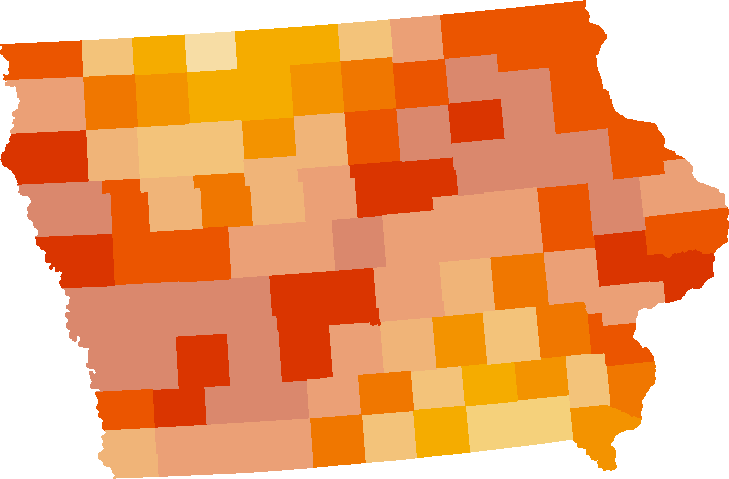
\includegraphics[keepaspectratio]{paper_files/figure-pdf/fig-bivariate-1.pdf}}

}

\subcaption{\label{fig-bivariate-1}Low Variance Data}

\end{minipage}%
%
\begin{minipage}{0.33\linewidth}

\centering{

\pandocbounded{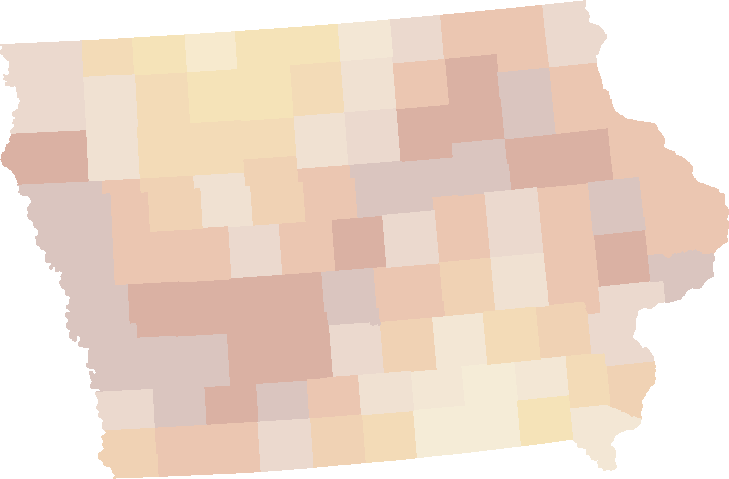
\includegraphics[keepaspectratio]{paper_files/figure-pdf/fig-bivariate-2.pdf}}

}

\subcaption{\label{fig-bivariate-2}High Variance Data}

\end{minipage}%
%
\begin{minipage}{0.33\linewidth}

\centering{

\pandocbounded{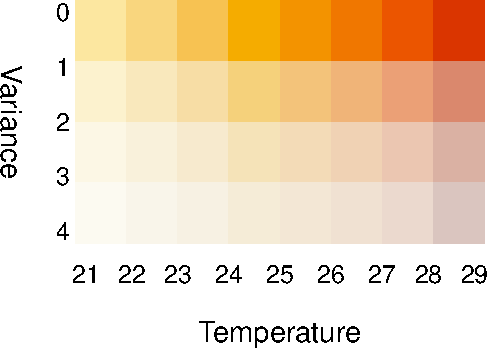
\includegraphics[keepaspectratio]{paper_files/figure-pdf/fig-bivariate-3.pdf}}

}

\subcaption{\label{fig-bivariate-3}Bivariate Palette}

\end{minipage}%

\caption{\label{fig-bivariate}A bivariate map that depict the counties
of Iowa where each county is coloured acording to it's average daily
temperature and the variance in temperature. This map is a choropleth
map with a two dimensional colour palette where temperature is
represented by colour hue, and variance is represented by colour
saturation. Even though uncertainty has been added to the graphic the
spatial trend is still clearly visible in the high variance case.}

\end{figure}%

\subsection{Why this approach may (or may not)
work}\label{why-this-approach-may-or-may-not-work}

The difficulty in incorporating uncertainty into a visualisation is
frequently mentioned but seldom explained. For example
\citet{Hullman2016} commented that it is straightforward to show a value
but it is much more complex to show uncertainty but did not explain why.
Many authors seem to believe uncertainty visualisation is a simple
high-dimensional visualisation problem, as the difficulty comes from
working out how to add uncertainty into already existing graphics
\citep{Griethe2006}. While this is part of the problem in uncertainty
visualisation, it is not the complete picture.
Figure~\ref{fig-bivariate} makes it clear that simply including
uncertainty as a variable is insufficient to perform signal-suppression.
If we cannot treat uncertainty the same as we would any other variable,
how should we treat it? We need to understand what uncertainty actually
\emph{is}, in order to understand how to integrate it into a
visualisation.

\subsubsection{It's a variable\ldots{} it's metadata\ldots{} it's
uncertainty?}\label{its-a-variable-its-metadata-its-uncertainty}

Describing what uncertainty actually is, is surprisingly hard. Most
authors simply avoid the problem and describe the characteristics of
uncertainty, of which there are plenty. Often, uncertainty is split
using an endless stream of ever changing boundaries, such as whether the
uncertainty is due to true randomness or a lack of knowledge
\citep{Spiegelhalter2017, Hullman2016, utypo}, if the uncertainty is in
the attribute, spatial elements, or temporal element of the data
\citep{Kinkeldey2014}, whether the uncertainty is scientific
(e.g.~error) or human (e.g.~disagreement among parties)
\citep{Benjamin2018}, if the uncertainty is random or systematic
\citep{Sanyal2009}, statistical or bounded
\citep{Gschwandtnei2016, Olston2002}, recorded as accuracy or precision
\citep{Griethe2006, Benjamin2018}, which stage of the data analysis
pipeline the uncertainty comes from \citep{utypo}, how quantifiable the
uncertainty is \citep{Spiegelhalter2017, utypo}, etc. There are enough
qualitative descriptors of uncertainty to fill a paper, but, none of
this is particularly helpful in understanding how to integrate it into a
visualisation. Rather than trying to define uncertainty by looking at
the myriad ways in which it \emph{does} appear in an analysis, we may
find it easier to look at where it \emph{does not}.

Descriptive statistics describe our sample as it is and summarises large
data down into an easy to swallow format. Descriptive statistics are not
seen as the primary goal of modern statistics, however, this was not
always the case. In 19th century England, \emph{positivism} was the
popular philosophical approach to science (positivists included famous
statisticians such as Francis Galton and Karl Pearson). Practitioners of
the approach believed statistics ended with descriptive statistics as
science must be based on actual experience and observations
\citep{Otsuka2023}. In order to make statements about population
statistics, future values, or new observations we need to perform
inference, which requires the assumption of the ``uniformity of
nature'', that is, we need to assume that unobserved phenomena should be
similar to observed phenomena \citep{Otsuka2023}. Positivists believed
referencing the unobservable was bad science. In other words, these
scientists embraced descriptive statistics due to the inherent certainty
that came with them. Since uncertainty is non-existent in descriptive
statistics, it is clear that uncertainty is a by-product of inference.

This history lesson illustrates what uncertainty actually is. At several
stages in a statistical analysis, we will violate the uniformity of
nature assumption. Each of these violations will impact the statistic we
have calculated and push it further from the population parameter we
wish to draw inference on. Uncertainty is the amalgamation of these
impacts. If we do not violate the uniformity of nature assumption at any
point in our analysis, we do not have any uncertainty.

This interpretation of uncertainty indicates that the uncertainty is not
a variable of importance in of itself. Uncertainty is metadata about our
statistic that is required for valid inference. This means uncertainty
should not be visualised by itself and we should seek to display signal
and uncertainty together as a ``single integrated uncertain value''
\citep{Kinkeldey2014}. This aspect of uncertainty visualisation makes it
a uniquely difficult problem.

\subsubsection{Visualising the ``single integrated uncertain
value''}\label{visualising-the-single-integrated-uncertain-value}

Typically, when making visualisations, we want the visual channels to be
separable. That is, we don't want the data represented through one
visual channel to interfere with the others \citep{Smart2019}. Mapping
uncertainty and signal to separable channels allows them to be read
separately, which does not align with the goal of communicating them as
a single integrated channel. Visualising uncertainty and signal
separately allows the uncertainty information to simply be ignored,
which is a pervasive issue in current uncertainty visualisation methods
\citep{uncertchap2022}. We can see this problem in
Figure~\ref{fig-bivariate}, as it sends the message ``this data has a
spatial trend and the estimates have a large variance'' as we read the
signal and the uncertainty separately.

This means effective uncertainty visualisation should be leveraging
integrability. That is, the visual channels of the uncertainty and the
signal would need to be separately manipulable, but read as a single
channel by the human brain. While most visual aesthetics \emph{are}
separable, there are some variables that have been shown to be
integrable, such as colour hue and brightness \citep{Vanderplas2020}.
When visualising uncertainty using its own visual channel, we can also
consider visual semiotics and make sure to map uncertainty to intuitive
visual channels, such as mapping more uncertain values to lighter
colours \citep{Maceachren2012}. Unfortunately relying on integrability
may not give us the amount of control we want over our
signal-suppression. Without a strong understanding of how these visual
channels collapse down into a single channel, relying on integrability
could create unintended consequences such as displaying phantom signals
or hiding justified signals. Additionally, multi-dimensional colour
palettes can make the graphics harder to read and hurt the accessibility
of the plots \citep{Vanderplas2015}.

There is another benefit to mapping uncertainty to saturation that is
not directly related to integrability. As the saturation decreases
colours become harder to distinguish. This means high uncertainty values
are harder to differentiate than low uncertainty values. We can leverage
this implicit feature of colour value by transforming the visual feature
space ourselves.

\section{Combining uncertainty and signal in a transformed
space}\label{combining-uncertainty-and-signal-in-a-transformed-space}

Instead of hoping that uncertainty might collapse signal values into a
single dimension, we can do some of that work ourselves. As a matter of
fact, some uncertainty visualisation authors already have.

\subsection{Value Suppressing Uncertainty
Palettes}\label{value-suppressing-uncertainty-palettes}

The Value Suppressing Uncertainty Palette (VSUP) \citep{Correll2018},
was designed with the intention of preventing high uncertainty values
from being extracted from a map. Since the palette was designed with the
extraction of individual values in mind and it has only been tested on
simple value extraction tasks \citep{Correll2018} or search tasks
\citep{Ndlovu2023}, it is unclear how effective the method is at
suppressing broader insights such as spatial trends.

Figure~\ref{fig-vsup} is a visualisation of the Iowa temperature data
using a VSUP to colour the counties. The low uncertainty case still has
a visible spatial trend, while the spatial trend in the high uncertainty
map has functionally disappeared. This means the VSUP has successfully
suppressed the spatial trend in the data. However, the spatial trend may
not be the only signal of concern in our graphic. Now we must return to
the original signal-suppression criteria and ask ourselves if they have
all been met. Are all the justified signals reinforced, while all the
unjustified signals are suppressed? Is a graphic that performs perfect
signal-suppression even possible?

\begin{figure}

\begin{minipage}{0.33\linewidth}

\centering{

\pandocbounded{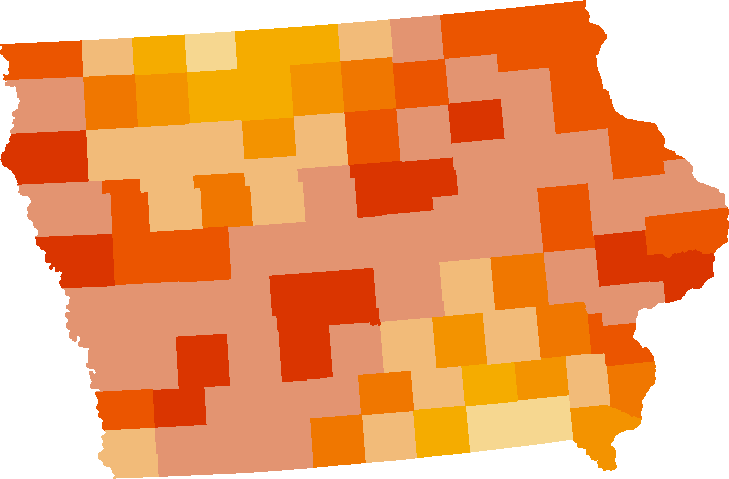
\includegraphics[keepaspectratio]{paper_files/figure-pdf/fig-vsup-1.pdf}}

}

\subcaption{\label{fig-vsup-1}Low Variance Data}

\end{minipage}%
%
\begin{minipage}{0.33\linewidth}

\centering{

\pandocbounded{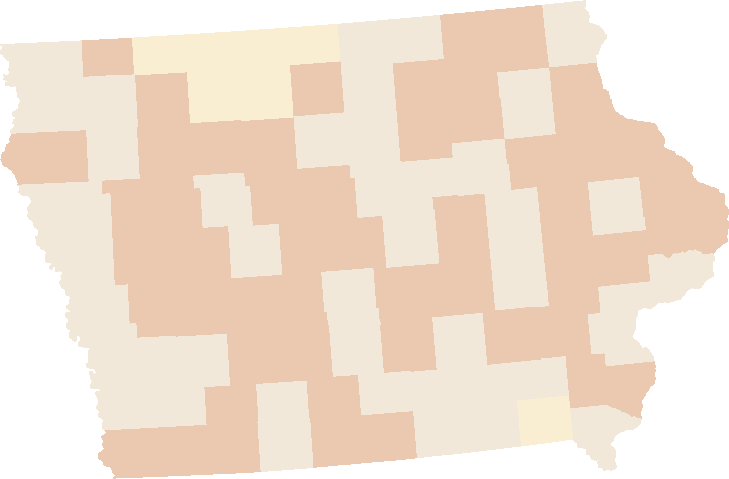
\includegraphics[keepaspectratio]{paper_files/figure-pdf/fig-vsup-2.pdf}}

}

\subcaption{\label{fig-vsup-2}High Variance Data}

\end{minipage}%
%
\begin{minipage}{0.33\linewidth}

\centering{

\pandocbounded{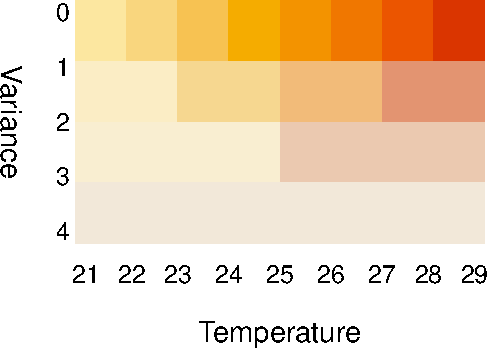
\includegraphics[keepaspectratio]{paper_files/figure-pdf/fig-vsup-3.pdf}}

}

\subcaption{\label{fig-vsup-3}VSUP Palette}

\end{minipage}%

\caption{\label{fig-vsup}A map made with a VSUP. The counties of Iowa
are coloured acording to its average daily temperature and the variance
in temperature. Similar to the bivariate map, temperature is mapped to
hue while variance is mapped to saturation. Unlike the bivariance map,
the colour space we are mapping our variables to has been transformed so
that high variance estimates are harder to discern from each other. This
map successfully reduces the visibility of the spatial trend in the high
uncertainty case while maintaining the visibility of the spatial trend
in the low uncertainty case.}

\end{figure}%

\subsection{What can and cannot be
suppressed?}\label{what-can-and-cannot-be-suppressed}

The methods used by the VSUP bring to light a slight problem with
uncertainty visualisation. Specifically, uncertainty and the purpose of
visualisation are somewhat at odds with one another. There are two
primary motivations behind visualisation, communication and exploratory
data analysis (EDA). Communication involves identifying a signal we want
to communicate and designing a visualisation that best conveys that,
while EDA involves creating a versatile visualisation and using it to
extract several signals. If we are designing an uncertainty
visualisation for communication then we can just suppress the specific
signal we are seeking to communicate. In the map example, we would
consider Figure~\ref{fig-vsup} to be a success as the only signal we are
concerned with is the spatial trend. However, it is not uncommon for
authors to express a desire for uncertainty visualisations that perform
signal-suppression in visualisations made for EDA
\citep{Sarma2024, Griethe2006}. For uncertainty visualisation for EDA to
work, we would need to assume that suppressing individual estimates
using their variance should naturally extend to broader suppression of
plot level insights. Unfortunately, it is unclear how reliably this
would work.

\subsubsection{There is no uncertainty in
EDA}\label{there-is-no-uncertainty-in-eda}

Earlier we established that uncertainty is a by-product of inference,
which means without inference, there is no uncertainty. Often EDA is
used to give us an understanding of our data and identify which signals
are worth pursuing. In this sense, EDA is the visual parallel to
descriptive statistics, as it is performed without an explicit
hypothesis, which means there is no inference, and by extension, there
is no uncertainty.

Some authors recognise inference will always occur (in some shape or
form) and believe uncertainty \emph{should} be visualised but do not
recognise \emph{how} uncertainty would be visualised.
\citet{Hullman2021} argued that there is no such thing as a
``model-free'' visualisation, therefore all visualisations require
uncertainty as we are always performing inference. While it is true that
we can think of visualisations as containing implicit inferential
properties, there are many potential inferences in any single
visualisation. This makes it a little difficult to ensure uncertainty is
always included. For example, if we have a visualisation that shows an
average, we would need to identify if the signal suppression should be
performed using the sampling variance or the sample variance
\citep{Hofman2020}. The distribution we use depends on the inferential
statistic but until the viewer chooses one and thinks about it (which
isn't easily observable), the particular variety of uncertainty which
would need to be displayed can't be calculated. This means the ideal
uncertainty visualisation should not only meet the signal suppression
requirements, but should also endeavor to be versatile enough to meet
those requirements for all the signals displayed in the graphic.

\subsubsection{The limitations of explicitly visualising uncertainty and
signal}\label{the-limitations-of-explicitly-visualising-uncertainty-and-signal}

The lack of versatility of the VSUP is easy to see with a simple
example.

Let's say we have a graphic that depicts a set of coefficients from a
linear regression and the value of the coefficient is shown using a
single colour. We want to know ``Which of these coefficients are
different from 0?'' as well as ``Which of these coefficients are
different from each other?''. To answer this question we do a series of
\(t\)-tests on these estimates. All of the individual \(t\)-tests of
fail to reject the null hypothesis that the coefficients are different
from 0. We then make a visualisation that suppresses this signal and
ensures that all of the estimates are visually indistinguishable from 0.
Next, we conduct two sample \(t\)-test and find that several of the
values need to be visually distinguishable from each other. The VSUP
method must pick a single colour for each estimate, and these colours
must be \emph{either} visually distinguishable or indistinguishable from
each other. We cannot perform signal-suppression on both these signals
simultaneously.

This example highlights a fundamental problem with the VSUP that extends
to the bivariate map as well. When we blend these colours, we need to
decide at what level of \emph{uncertainty} to blend these colours
together. Even though the bivariate map does not explicitly combine
colour values at certain variance levels, the mapping of variance to
colour saturation does this implicitly. That is, at certain saturation
values the colours in a bivariate map are imperceptibly different and
appear as though they are mapped to the same value. At this point, it is
irrelevant whether or not the colours are technically different, they
are the same colour in the human brain. This is of course complicated by
the fact that human colour perception varies at an individual level.
Some women are believed to have four different cone cells which allows
them to perceive a greater range of colours, while others only have one
or two types of cone cells and have colour deficiencies
\citep{simunovic2010} For VSUP to function for all individuals, we must
calibrate each plot to an individual's ability to perceive colour.

If we only use a single colour to express each signal-suppressed
statistic, we will always need to decide which signals we suppress and
which we do not. This issue has already been raised in the literature.
Which hypothesis are suppressed and which are not largely depends on the
method used to combining colours in the palette \citep{Kay2019}. The
VSUP in Figure~\ref{fig-vsup} used the tree based method that was used
by \citet{Correll2018}, but there are alternatives that are more
appropriate for different hypothesis.

Uncertainty visualisation for EDA would be possible if we designed a
plot in such a way that suppressing individual estimates using their
variance would naturally extend to broader suppression of plot level
insights. This assumption is commonly made by visualisation researchers
in normal visualisation experiments \citep{North2006}. If we could
express the statistic of a cell using multiple colours, this limitation
may disappear entirely.

\section{Implicitly Combining Uncertainty and
Signal}\label{implicitly-combining-uncertainty-and-signal}

Rather than trying to figure out how to combine signal and uncertainty
into a single colour, we can just display a sample instead and allow the
viewer to extract \emph{both} the estimate and the variance.

\subsection{Pixel map}\label{pixel-map}

Figure~\ref{fig-pixel} displays a pixel map \citep{Lucchesi2021}, which
is a variation of the choropleth map where each area is divided up into
several smaller areas, each coloured using outcomes from the larger
area's (i.e.~the county's) average temperature sampling distribution.
The spatial trend is clearly visible in the low variance case, but
functionally disappears in the low variance case. While the spatial
trend is just barely visible in the high uncertainty case, it is much
harder to see. This means the graphic also achieves the third criteria
for signal-suppression, i.e.~our difficulty in seeing the distribution
is proportional to the level of uncertainty in the graphic.

\begin{figure}

\begin{minipage}{0.33\linewidth}

\centering{

\pandocbounded{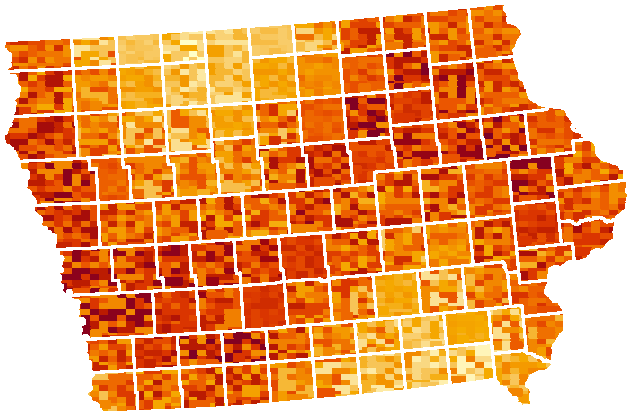
\includegraphics[keepaspectratio]{paper_files/figure-pdf/fig-pixel-1.pdf}}

}

\subcaption{\label{fig-pixel-1}Low Variance Data}

\end{minipage}%
%
\begin{minipage}{0.33\linewidth}

\centering{

\pandocbounded{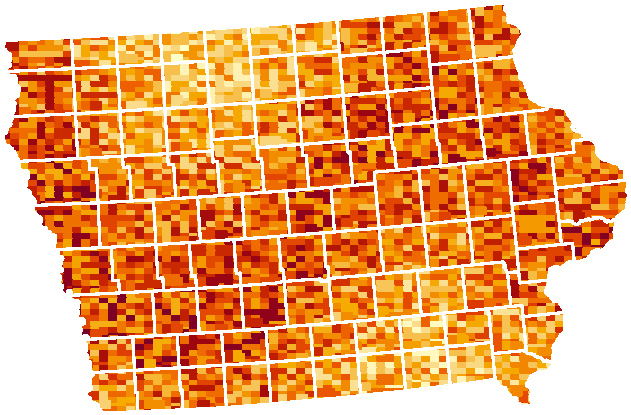
\includegraphics[keepaspectratio]{paper_files/figure-pdf/fig-pixel-2.pdf}}

}

\subcaption{\label{fig-pixel-2}High Variance Data}

\end{minipage}%
%
\begin{minipage}{0.33\linewidth}

\centering{

\pandocbounded{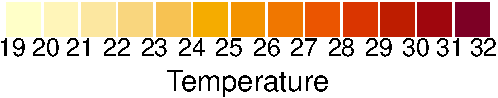
\includegraphics[keepaspectratio]{paper_files/figure-pdf/fig-pixel-3.pdf}}

}

\subcaption{\label{fig-pixel-3}Pixel Map Palette}

\end{minipage}%

\caption{\label{fig-pixel}A pixel map of the counties of Iowa. In this
map, each county is broken up into several small areas and coloured
according to a potential daily temperature, given the its average daily
temperature and its sampling distribution. This results in each county
being represented by a sample rather than a single value. In this
graphic, we can clearly see the spatial trend in the low variance case,
while the spatial trend is much harder to identify in the high variance
case.}

\end{figure}%

It is clear that the pixel-map is not only suppressing the false
information, but it is doing so by simulating \emph{more} information.
The efficacy of this method means that visualisations of simulated
samples pop up repeatedly in the literature, with examples including
samples that are animated over time \citep{Hullman2015, Blenkinsop2000},
pixel-maps, and spaghetti time series plots. Not only does this method
help readers understand the plot level gist, it is also unlikely to
damage the viewers ability to extract individual estimates. Extracting
global statistics, such as the mean or variance, from a sample can be
done with relative ease, especially when those values are mapped to
colour \citep{Franconeri2021}. Additionally, \citet{Ndlovu2023} found
that participants applied the same methods they used for simple
choropleth maps to complicated uncertainty maps even if that take away
was invalid. The pixel map can be read the same way as a choropleth map,
which allows us to leverage that automatic response. Therefore, the
pixel map performs signal suppression, without sacrificing the viewers
ability to extract general statistics, unless those statistics
\emph{should} be harder to extract due to the uncertainty in the value.
So, what is it about Figure~\ref{fig-pixel} that allows it to be such a
successful uncertainty visualisation? Is this a question we can easily
answer?

\subsection{Show me the data}\label{show-me-the-data}

To thoroughly understand why pixel maps seem to successfully perform
signal suppression, we would need a more thorough discussion than what
can be offered here. However, this does not prohibit us from discussing
potential reasons for the graph's effectiveness. There is a second type
of uncertainty that the pixel map quietly communicates but we have not
touched on yet, and this uncertainty is also conveyed by visualisations
of our raw data. That is, these graphics can show assumption violations.

As we discussed in previous sections, we can consider uncertainty to be
``the amalgamations of the impacts of violations to the assumption of
the uniformity of nature''. It's not a definition that rolls off the
tongue, but we can work with it. Thankfully, this definition of
uncertainty aligns nicely with all the concepts that are included in the
uncertainty umbrella. Some works
\citep{Hullman2018, Maceachren2012, Thomson2005} focus narrowly on
specific terms with mathematical definitions, such as probability,
confidence intervals, variance, error, or precision. These works are
only concerned with quantifying the final impact of uncertainty on our
statistics. That is, how large should the bound around our statistic be,
such that our ``true'' statistic can be inferred. Others
\citep{Griethe2006, Leland2005, Pang1997, Pham2009, Boukhelifa2017}
include broader loosely related elements, such as missing values,
reliability, model validity, or source integrity. These broader and
harder to quantify concepts are concerned about potential sources of
uncertainty, that is, they describe violations to the assumption of the
uniformity of nature.

What this means is that we have two types of uncertainty, but one is
more ``processed'' than the other. Quantifiable uncertainties are just
assumption violations expressed as an effect on our final statistic (or
true variation of our data). The disconnect between quantifiable and
unquantifiable uncertainty creates a huge problem for authors trying to
visualise it. A survey of visualisation authors cited ``not knowing how
to calculate uncertainty'' as one of the primary reasons they did not
include it in visualisations \citep{Hullman2020a}.

There are two reasons we might leave our uncertainty as an assumption
violation rather quantifying the effect. The first reason is that we may
be unable to translate the assumption violation to a quantifiable
uncertainty. There is no blanket rule that allows us to reliably
quantify all uncertainty for every statistic, although some researchers
have tangled with the idea. For example, \citet{Thomson2005} suggests a
mathematical formula for \emph{examples} of uncertainty, and information
theory tries to quantify uncertainty using the idea of entropy, but they
ignore the disconnect between the broad concept of uncertainty and what
we can reliably quantify. Some authors don't believe that it is even
possible to quantify all the assumption violations
\citep{Spiegelhalter2017}.

The second reason to leave uncertainty as a potential violation of our
assumptions, is that we might not know the final statistic we are
seeking to calculate. This is the case for visualisations made for EDA,
and a large number of developments in EDA visualisation have been in
displaying these difficult to quantify violations. For example,
\citet{Tierney2023} builds upon the tidy data principles to allow users
to handle missing values. This includes data plots with a missing value
``shadow'' that allows visualisation authors to identify if the
variables used in a plot have any structure in their missing values,
which would contribute to uncertainty.

With this understanding it becomes clear to see why uncertainty is tied
to an endless string of examples in the data analysis pipeline.
Uncertainty examples include imputed data, model selection, inherent
randomness, biased sampling, etc., not because these things \emph{are}
uncertainty, but because they \emph{create} uncertainty when we perform
inference. Whether or not these elements are relevant is highly
dependent on what statistic you are trying to draw inference on, and by
extension, the purpose of your visualisation.

This relationship between uncertainty and the purpose of our analysis is
littered throughout the literature. Multiple authors have commented on
the need to consider quantifying and expressing uncertainty at every
stage of a project as the goal shapes every step of the analysis
\citep{Kinkeldey2014, Hullman2016, Refsgaard2007}. \citet{Otsuka2023}
suggested that the process of observing data to perform statistics is
largely dependent on our goals, because the process of boiling real
world entities down into probabilistic objects (or ``probabilistic
kind'' as he puts it) depends on the relationship we seek to identify
with our data. \citet{Meng2014} commented what is kept as data and what
is tossed away is determined by the motivation of an analysis and what
was previously noise can be shown to become signal depending on the
question we seek to answer.\\
\citet{Wallsten1997} argue that the best method for evaluating or
combining subjective probabilities depends on the uncertainty the
decision maker wants to represent and why it matters.
\citet{Fischhoff2014} looks at uncertainty visualisation for decision
making decides that we should have different ways of communicating
uncertainty based off what the user is supposed to do with it.

This makes it very difficult to move quantified uncertainty through the
layers of our analysis, especially when designing a visualisation for
EDA. If we don't know what the final statistic is, we cannot quantify
the effects of our assumptions. Therefore, it is often the case that the
best uncertainty visualisation is not an uncertainty visualisation at
all, but simply the most accurate depiction of our raw data. This does
not mean that visualising raw data will always prevent insignificant
signal from getting through. \citet{Chowdhury} illustrated how groups
that appear linearly separable in a linear discriminant analysis (LDA)
visualisation of the data can actually be the result of a LDA performed
on too many variables, something that was not clear from the
visualisation until the line-up protocol was implemented. However, just
showing the data is a simple but effective option for uncertainty
visualisation that seems to be largely overlooked.

Of course, visualising the raw data is not always possible nor suitable.
For example, if we have a specific statistic in mind, it may be more
appropriate to show the sampling distribution of that statistic rather
than the variability of all observations. If we visualise that sampling
distribution in a way that allows us to see it's shape, and therefore
recognise any assumption violations (such as a non-normal distribution),
we maintain some of the benefits that came with visualising the raw
data. This is exactly what the pixel map does, and likely contributes to
it's success as a signal suppression method.

\section{Evaluating uncertainty
visualisations}\label{evaluating-uncertainty-visualisations}

If we want to make conclusions about how effective any uncertainty
visualisation method is we need to look at the results of evaluation
experiments. Unfortunately the illustrative methods we have used thus
far, i.e.~showing a graphic and saying ``wow look at this'', is lacking
if we want any serious results. However, despite the abundance of
uncertainty visualisation evaluation experiments, existing literature
reviews have struggled to synthesise them into any common rules
\citep{Kinkeldey2014, Hullman2016}.

Here we discuss common evaluation methods, why these methods might
struggle to create a cohesive set of recommendations for uncertainty
visualisations, and consider how to evaluate visualisations on their
ability to perform signal-suppression.

\subsection{Current methods}\label{current-methods}

Including uncertainty in a visualisation comes with many secondary
benefits. Examples of these benefits include better decisions, more
trust in the results and the ability to extract additional statistics,
such as the variance. Ultimately, these secondary benefits are not the
primary goal of uncertainty visualisation, and evaluating uncertainty
visualisations on these criteria often has unintended consequences.

\subsubsection{Value extraction of uncertainty
statistics}\label{value-extraction-of-uncertainty-statistics}

Uncertainty visualisations are often evaluated based on how accurately
\citep{Hullman2019} viewers can separately extract the estimate and its
variance \citep{Kinkeldey2014}. This means a significant chunk of
evaluation studies boil down to showing a participant a visualisation
and asking questions such as ``what is the variance of \(X\)?'', or
``what is the mean of \(X\)?''. This seems like a relatively straight
forward approach, and it is similar to how non-uncertainty
visualisations are evaluated, but is this appropriate for uncertainty
visualisations? The role of uncertainty is rarely evaluated in these
studies as the graphics are often compared on the basis of being
uncertainty visualisations \citep{Ibrekk1987, Hullman2015, Hofman2020},
a class that has no established definition. By shifting the focus of our
inference from \(\bar{X}\) to \(Var(X)\) or \(P(X)\) we end up
evaluating visualisations on their ability to convey uncertainty
statistics, rather than on uncertainty's ability to suppress statistics.
This leads to a series of experiments where the uncertainty is evaluated
as a signal even if that was not the goal of the experiment.

The problem with evaluating uncertainty as a signal are identical to the
problems associated with displaying uncertainty as a signal. There is no
reason to assume uncertainty would behave any differently to any other
variable when we evaluate them in this way. For example,
\citet{Ibrekk1987} found that participants were more accurate at
extracting a statistic when it could be directly read off the graphic,
than when it required an area estimate (which is the case if using the
probability density function), or when there was no visual indicator for
the statistic at all (which is the case when using the cumulative
distribution function of a skewed random variable). \citet{Hullman2015}
found that a visualisation that allows viewers to count outcomes to
estimate a probability outperformed one that required a complicated area
calculation. \citet{Hofman2020} and \citet{Zhang2022} found that
participants were better at answering questions about prediction
intervals when shown a prediction interval instead of a sampling
distribution. \citet{Gschwandtnei2016} found that graphics where the
required statistic could be directly read off the plot outperformed
those that involved guesswork due to a gradually decreasing line.
\citet{Cheong2016} found that participants made better decisions when
they were explicitly given the relevant probability in text rather than
when they needed to read it off a map. It is well established that
extracting information from a graphic using a perceptual task will
always be less accurate than explicitly reading the value provided in
text form \citep{Cleveland1984}.

The biggest failing of this evaluation method is not the predictable
outcomes, but that it encourages us to see successful examples of
signal-suppression as a failing. \citet{Blenkinsop2000} commented that
visually integrable depictions of uncertainty should be avoided, as they
decrease the viewers confidence in their extracted data values. This
conclusion is antithetical to the goals of signal-suppression and occurs
because these methods evaluate uncertainty as a signal, not as noise.

\subsubsection{Trust, confidence, and risk
aversion}\label{trust-confidence-and-risk-aversion}

Trust is a by-product of displaying uncertainty so it is commonly
measured in uncertainty evaluation studies \citep{Hullman2019}.
Considering trust, and not transparency, as the metric of importance in
uncertainty communication can lead to a questionable subtext that argues
against transparency, something that has been noticed by several other
authors \citep{Spiegelhalter2017, ONeill2018}. Science communication
should be primarily concerned with accuracy. This accuracy may not
always involve showing the data exactly as it is, for example we may
want to adjust our graphic to correct for visual heuristics, but these
changes should still be in pursuit of accuracy. Setting trust as the
variable of interest implicitly encourages statisticians to set trust as
the primary goal of communication. Evaluating visualisations on trust
conflates trust and transparency and ultimately discourages
signal-suppression. We can see this effect pop up in the results of
evaluation studies. For example, \citet{Zhao2023} found that
participants were more trusting of model estimates with low uncertainty,
but this effect did not carry over to estimates with high uncertainty.
Despite decreased trust being a desired outcome of signal suppression,
the author's discussion implied this result was not desired. This
perspective ends up extending to visualisation authors as well.
\citet{Hullman2020a} found that authors simultaneously argued that
failing to visualise uncertainty was akin to fraud, but also many
avoided uncertainty visualisation because they didn't want their work to
come across as untrustworthy. This is a classic example of the negative
impacts of placing direct importance on \emph{trust} rather than
\emph{transparency}. In cases of high uncertainty, authors will opt to
leave out uncertainty information because it decreases confidence in the
authors conclusions. This is the end result of designing uncertainty
visualisations for increased trust, rather than signal-suppression. Of
course, this does not mean measuring trust or perceived trustworthiness
has no place in visualisation experiments. After all, if participants
political motivations can influence their ability to accurately read a
plot \citep{nurse2020}, then their level of trust in the information
could have a similar effect. However, it does mean trust should not be
the primary goal of uncertainty visualisation evaluation experiments.

Another metric that is similar to trust is the participants confidence
in their decision or extracted value. Confidence has many of the same
issues as trust, but it has an additional confounding factor. In
non-uncertainty visualisation evaluation experiments, confidence is used
as a proxy for the clarity of the visualisation. Confidence cannot
simultaneously be a measure of clarity of visualisation \emph{and} a way
to capture the uncertainty expressed in a visualisation. Uncertainty
visualisations conflate these two measures.

Risk-aversion is another secondary effect of uncertainty visualisation
that is used to evaluate uncertainty visualisations \citep{Hullman2019}.
Risk aversion is an economics term used to describe an agent who would
chose a random variable with a lower expected payout because it also has
a lower variance. Risk aversion is considered irrational behaviour
because it is a deviation from the behaviour of a rational agent.
Comparing participant responses to that of a rational agent has even
been suggested as a benchmark for uncertainty visualisation experiments
\citep{wu2023rational}. However, just like trust, evaluating graphics on
risk-aversion discourages signal-suppression. Rational agents \emph{by
definition} should \emph{ignore} uncertainty information. Risk aversion
is considered to be irrational because it means the economic agent
\emph{is} considering the uncertainty information. The only case where a
rational agent should not ignore the uncertainty information is when the
uncertainty is signal, not noise. Designing graphics that encourage
choices that align with that of a rational agent, is to encourage
graphics that do not include uncertainty at all.

For these reasons we do not believe trust, confidence, or risk-aversion
are useful measures to evaluate uncertainty visualisations. While they
are designed to capture the secondary effects of uncertainty, using them
as primary measures of visualisation performance is in direct conflict
with designing visualisations for signal-suppression.

\subsubsection{Questions that attempt to capture
signal-suppression}\label{questions-that-attempt-to-capture-signal-suppression}

There is a collection of studies that seem to be aware of the issues
behind using trust or value extraction to evaluate uncertainty
visualisations. These studies try to measure the effect of some kind of
single integrated value, but the methodology is often ad-hoc with
varying levels of success.

The first method is what we call the ``vague question'' approach. The
authors of these studies will ask the participants a question that
implies that they should use the uncertainty information, but it is
unclear how. The authors then go on to compare the readers answer to a
very specific ground truth. This means the participants are being
\emph{evaluated} as though they are performing a value extraction task,
but they are not being asked the \emph{questions} that are asked in the
value extraction task. Ultimately this approach results in strangely
cryptic questions that create a large amount of noise due to the varied
interpretation of the questions \citep{Hullman2016}.

For example \citet{Hofmann2012} showed study participants 20 plots,
where each plot displayed two distributions (as a pair of jittered
samples, density plots, histograms, or box plots) and asked them to
identify the plot where ``the blue group is furthest to the right''. The
mean of the two groups was used to decide which group was actually
``furthest to the right'' and the different graphical approaches were
evaluated against that ground truth. In another example
\citet{Ibrekk1987} asked participants for the ``best estimate'', but the
participant's responses were evaluated against the mean of the
distribution. Ultimately, the term ``best'' is up to the users
interpretation, and the estimate that minimised the sum of squared
errors was not implied by the question. This vague question approach
leads to inconclusive results, as we are left unclear if it was the
phrasing of the question or the plot design that caused the participants
to answer incorrectly.

A variation of the vague question problem, is a series of studies that
ask questions that are impossible to answer using the information given
to the participants. These studies frequently expect participants to
give deterministic answers for probabilistic questions. For example
\citet{Correll2014} showed participants the distribution of voter
preferences for two candidates in an election, and asked them ``how
likely is candidate B to win the election?''. Participants were not able
to answer the question about likelihood in term of probability, but were
instead given seven options from 1 = ``Outcome will be most in favour of
A'' to 7 = ``Outcome will be most in favour of B''. The ground truth
statistic for this question was a scalar multiple of Cohen's d,
indicating participants were supposed to incorporate uncertainty
information using a very specific formula that was likely unknown to
them but assumed to be used implicitly.\\
In another example, \citet{Padilla2017} provided participants with a
visualisation of the cone of uncertainty and asked then to ``decide
which oil rig will receive more damage based on the depicted forecast of
the hurricane path''. The cone of uncertainty provides a 60\% confidence
interval for the location of the eye of a hurricane, which allows us to
know the area where the eye of the storm will go, but it does not given
any information about the intensity of a storm, the size of a storm, or
even if a location will be hit. Other authors have commented on the
complexity of communicating hurricane risk because the path, storm surge
and wind speed are all important and cannot be ignored
\citep{Spiegelhalter2017}. \citet{Padilla2017} seem to be aware of the
issues in the visualisation and are using the user study to show that
current government communications are not the best choice when
communicating hurricane risk, as it is unreasonable to assume that
``more likely to be hit'' should automatically translate to ``more
damage''. While this is useful to highlight, the authors end up caught
by their own trap, as answering the questions in their second study
correctly required participants to assume an area being more likely to
be hit \emph{does} translate to receiving more damage. The assumptions
required to answer these deterministic questions are often invisible,
even to the authors of the paper, which means they often create more
problems than they solve when they are used as a tool for graphical
evaluation. Similar to the vague question problem, these studies seem to
be aware that we should be evaluating an uncertainty visualisation based
on a deterministic observation (such as our example of ``does this map
have a spatial trend'') but are unsure how to incorporate or evaluate
it.

While these approaches are certainly a step in the right direction, the
experiments end up having far too much noise in their results. This is
further complicated by the fact that visual statistics and their
computational equivalents often differ, even before we consider these
measurement errors. By having a ground truth, these experiments
implicitly ask users to treat uncertainty as a signal which goes against
the purposes of signal-suppression.

\subsection{Testing signal
suppression}\label{testing-signal-suppression}

If we cannot ask direct questions about uncertainty, or measure the
secondary effects of uncertainty, or ask indirect questions about the
uncertainty; then how are we supposed to evaluate uncertainty
visualisations? How do you measure something that disappears the second
you look directly at it? To evaluate uncertainty visualisations, we need
an experimental design that evaluates uncertainty as noise, not as
signal. This means we need to measure \emph{uncertainty's impact on the
signal}, not the uncertainty itself.

\subsubsection{Comparing to hypothesis
tests}\label{comparing-to-hypothesis-tests}

The most obvious way to evaluate uncertainty visualisations is to
compare the visualisations to statistical tests. If a graphic was
performing signal-suppression we would expect the signal to be harder to
see at higher levels of uncertainty. The ideal outcome is a an
uncertainty visualisation where the signal is only perceivable when it
would be identified by a hypothesis test. Evaluating visualisations as
though they are akin to hypothesis tests is a well established concept
in visualisation. The lineup protocol is a good example of this
approach. Lineups are a confirmatory visualisation tool that can be used
to check if perceived patterns are real or merely the result of chance
\citep{Buja2009, Wickham2010}. Lineups can also be used to evaluate the
effectiveness of different types of plots \citep{Hofmann2012} and design
decisions \citep{vanderplas2017}. The motivation behind the lineup
protocol is similar to the motivations behind signal-suppression,
although the lineup protocol is more explicitly tied to a specific
hypothesis. \citet{Patrick2023} compared standard statistical tests to
the lineup-protocol, and evaluated the visualisations using the power
curves that are typical for hypothesis testing. In a similar vein,
\citet{Kim2019} investigated how different uncertainty visualisation
methods influenced user's prior beliefs, and evaluated the graphics by
comparing their results to those from Bayesian inference. This approach
is similar to the lineup protocol as it also evaluates a visualisation
by comparing it to an analogous statistical calculation, however it does
so using a different statistical philosophy. The connection with
visualisation and statistical tests even extends to EDA, where
\citet{Hullman2021} commented that a visualisation can be considered a
model check where the null hypothesis is the expected and we are looking
for the unexpected. This is all to say that comparing visualisations to
hypothesis tests is not uncharted territory.

We could use a similar evaluation method to evaluate uncertainty
visualisations, however, it is not entirely clear what the computational
equivalent of an uncertainty visualisation is. Even the lineup protocol,
which is much closer to a standard statistical test, runs into some
difficulty when trying to directly compare it to its computational
equivalent. \citet{Patrick2023} found that human viewers using the
lineup protocol are less sensitive to deviations from the null
hypothesis than standard statistical tests. However, this finding does
not directly translate to the lineup protocol being worse than its
computational equivalent. The lineup protocol allows viewers to detect
if ``something'' is not right even if that something is unspecified, or
what the authors intended. For example, \citet{vanderplas2017} did an
experiment where participants were drawn to plots with unequal cluster
sizes, even though the size of the cluster was not one of the features
the authors were testing. While standard hypothesis tests may outperform
the lineup protocol on power, computational tests have the benefit of
knowing exactly what they are looking for. Visualisations are often
explicitly made when we \emph{don't} know what we are looking for.
Additionally, lineup protocols often have a specific hypothesis that is
used to create the null distribution, while uncertainty visualisations
are intended to be more flexible and can be created without identifying
a specific null distribution. Therefore, while we could evaluate
uncertainty visualisations by comparing them to a selection of
hypothesis tests, we should not expect the same level of sensitivity
that we get in standard hypothesis tests as the assumed knowledge about
our data is quite different. This approach could give us a good idea of
the use cases of different uncertainty visualisation designs, but we
should be mindful of it's limitations in fully describing the
effectiveness of these graphics.

\subsubsection{Qualitative Studies}\label{qualitative-studies}

Alternatively visualisation research could shift away from the accuracy
concept all together and ask questions that allow for open ended
responses. This method can enlighten authors as to \emph{how} the
uncertainty information was used by the participants.
\citet{Hofmann2012} captured this by asking participants why they
considered a particular plot to be more right-shifted, even though this
qualitative analysis did not make it into the final paper.
\citet{Daradkeh2015} presented participants with ten investment
alternatives and asked participants ``from among available alternatives,
which alternative do you prefer the most'', and were asked to think
aloud and consider the uncertainty in their decision making. The
experimenters goal was to observe and organise the methods people use
when making decisions in the face of uncertainty. They highlighted the
specific aspects of uncertainty that participants typically considered,
such as the range of outcomes that are above/below a certain threshold,
minimum and maximum values, the risk of a loss, etc., and identified
where in the decision making process participants made these
considerations.

\subsubsection{Heuristics}\label{heuristics}

While experiments that explicitly identify heuristics in current methods
are not technically measuring signal-suppression, they are still a
useful consideration to keep in mind when designing experiments for
signal suppression. Heuristic checks look at unknown pitfalls that might
exist in interpretation of current plots \citep{Hullman2016} and can
change depending on the larger scope of the graphic and the population
we are communicating with \citep{Spiegelhalter2017, Kinkeldey2014}.

Several heuristics are of particular importance for uncertainty
visualisations, and are likely to impact how well different methods
performing signal suppression. The sine illusion can cause the
confidence interval of a smoothed sine curve to seem wider at the peaks
than the troughs, causing us to underestimate uncertainty associated
with changing values \citep{Vanderplas2015}. Points that were on an
outcome of an ensemble display were perceived as more likely than points
not on an outcome, even when the point that was not on an outcome was
closer to the centre of the distribution (and therefore more likely)
\citep{Padilla2017}. This can be considered an extension of the within
bar bias, where participants looking at a bar chat with error bars view
outcomes within the bar as more likely than those outside it
\citep{Newman2012}. Several studies have found that viewers use a
heuristic where they compare the distance between two estimates to
estimate if they are different, and in doing so, ignore the uncertainty
information \citep{uncertchap2022}.

These heuristics have the potential to create noise in signal
suppression evaluations, and should be kept in mind when designing an
evaluation experiment.

\section{Conclusions and Future work}\label{conclusions-and-future-work}

This paper has identified gaps in the uncertainty visualisation
literature that must be filled for the field to progress. We formalised
the uncertainty visualisation problem, and in doing so highlighted an
untouched area of uncertainty visualisation research.

\emph{Experimental practices on uncertainty visualisation need to be
standardised.} Uncertainty visualisations for decision making treat
uncertainty as signal, while visualisations for signal-suppression treat
uncertainty as noise. As the literature currently exists, there is no
way to combine papers to get a meaningful sense of how uncertainty
information is understood by a viewer. Researchers need to ensure that
when they identify the motivation behind their visualisation technique,
and that their evaluation methods match the motivations of the paper.
Additionally \emph{evaluation methods that evaluate uncertainty as noise
need to be developed.}

\emph{Experimenters should consider evaluating visual aesthetics on how
well they suppress information in a graphic.} Research into separability
and integrability is of particular interest to uncertainty
visualisation, as it allows interference from the uncertainty variable.
When designing experiments, authors often choose aesthetics that are
visually distinguishable; uncertainty visualisation authors should
consider doing the opposite.

\emph{Software that allows users to easily perform signal suppression
should be developed.} Existing uncertainty visualisation methods view a
distribution as its own object and there are no software options for the
``an uncertainty visualisation is a function of an existing
visualisation'' philosophy.

Signal suppression is an untouched area of visualisation research and
developing methods for the practice may require us to challenge our
entire notion of what makes a good visualisation. We are interested to
see how this challenge plays out.

\section{Acknowledgements}\label{acknowledgements}

The first author of this paper is supported in part by a scholarship
from the the Australian Energy Market Operator. The R packages were used
for this work were: \texttt{tidyverse} \citep{tidyverse},
\texttt{Vizumap} \citep{Vizumap}, \texttt{RColorBrewer}
\citep{RColorBrewer}, \texttt{scales} \citep{scales}, \texttt{sf}
\citep{sf}, \texttt{ggrepel} \citep{ggrepel}, \texttt{urbnmapr}
\citep{urbnmapr}, \texttt{flextable} \citep{flextable},
\texttt{colorspace} \citep{colorspace}, and \texttt{rgeos}
\citep{rgeos}. The GitHub repository for this paper can be found at
https://github.com/harriet-mason/ARSA-UncertaintyLitReview which
contains the files required to reproduce this article in full.


\renewcommand\refname{Bibliography}
\bibliography{paper.bib}



\end{document}
